\documentclass[journal,12pt,twocolumn]{IEEEtran}

\usepackage{setspace}
\usepackage{gensymb}
\singlespacing
\usepackage[cmex10]{amsmath}

\usepackage{amsthm}

\usepackage{mathrsfs}
\usepackage{txfonts}
\usepackage{stfloats}
\usepackage{bm}
\usepackage{cite}
\usepackage{cases}
\usepackage{subfig}

\usepackage{longtable}
\usepackage{multirow}

\usepackage{enumitem}
\usepackage{mathtools}
\usepackage{steinmetz}
\usepackage{tikz}
\usepackage{circuitikz}
\usepackage{verbatim}
\usepackage{tfrupee}
\usepackage[breaklinks=true]{hyperref}
\usepackage{graphicx}
\usepackage{tkz-euclide}

\usetikzlibrary{calc,math}
\usepackage{listings}
    \usepackage{color}                                            %%
    \usepackage{array}                                            %%
    \usepackage{longtable}                                        %%
    \usepackage{calc}                                             %%
    \usepackage{multirow}                                         %%
    \usepackage{hhline}                                           %%
    \usepackage{ifthen}                                           %%
    \usepackage{lscape}     
\usepackage{multicol}
\usepackage{chngcntr}

\DeclareMathOperator*{\Res}{Res}

\renewcommand\thesection{\arabic{section}}
\renewcommand\thesubsection{\thesection.\arabic{subsection}}
\renewcommand\thesubsubsection{\thesubsection.\arabic{subsubsection}}

\renewcommand\thesectiondis{\arabic{section}}
\renewcommand\thesubsectiondis{\thesectiondis.\arabic{subsection}}
\renewcommand\thesubsubsectiondis{\thesubsectiondis.\arabic{subsubsection}}


\hyphenation{op-tical net-works semi-conduc-tor}
\def\inputGnumericTable{}                                 %%

\lstset{
%language=C,
frame=single, 
breaklines=true,
columns=fullflexible
}
\begin{document}

\newcommand{\BEQA}{\begin{eqnarray}}
\newcommand{\EEQA}{\end{eqnarray}}
\newcommand{\define}{\stackrel{\triangle}{=}}
\bibliographystyle{IEEEtran}
\raggedbottom
\setlength{\parindent}{0pt}
\providecommand{\mbf}{\mathbf}
\providecommand{\pr}[1]{\ensuremath{\Pr\left(#1\right)}}
\providecommand{\qfunc}[1]{\ensuremath{Q\left(#1\right)}}
\providecommand{\sbrak}[1]{\ensuremath{{}\left[#1\right]}}
\providecommand{\lsbrak}[1]{\ensuremath{{}\left[#1\right.}}
\providecommand{\rsbrak}[1]{\ensuremath{{}\left.#1\right]}}
\providecommand{\brak}[1]{\ensuremath{\left(#1\right)}}
\providecommand{\lbrak}[1]{\ensuremath{\left(#1\right.}}
\providecommand{\rbrak}[1]{\ensuremath{\left.#1\right)}}
\providecommand{\cbrak}[1]{\ensuremath{\left\{#1\right\}}}
\providecommand{\lcbrak}[1]{\ensuremath{\left\{#1\right.}}
\providecommand{\rcbrak}[1]{\ensuremath{\left.#1\right\}}}
\theoremstyle{remark}
\newtheorem{rem}{Remark}
\newcommand{\sgn}{\mathop{\mathrm{sgn}}}
\providecommand{\abs}[1]{\vert#1\vert}
\providecommand{\res}[1]{\Res\displaylimits_{#1}} 
\providecommand{\norm}[1]{\lVert#1\rVert}
%\providecommand{\norm}[1]{\lVert#1\rVert}
\providecommand{\mtx}[1]{\mathbf{#1}}
\providecommand{\mean}[1]{E[ #1 ]}
\providecommand{\fourier}{\overset{\mathcal{F}}{ \rightleftharpoons}}
%\providecommand{\hilbert}{\overset{\mathcal{H}}{ \rightleftharpoons}}
\providecommand{\system}{\overset{\mathcal{H}}{ \longleftrightarrow}}
	%\newcommand{\solution}[2]{\textbf{Solution:}{#1}}
\newcommand{\solution}{\noindent \textbf{Solution: }}
\newcommand{\cosec}{\,\text{cosec}\,}
\providecommand{\dec}[2]{\ensuremath{\overset{#1}{\underset{#2}{\gtrless}}}}
\newcommand{\myvec}[1]{\ensuremath{\begin{pmatrix}#1\end{pmatrix}}}
\newcommand{\mydet}[1]{\ensuremath{\begin{vmatrix}#1\end{vmatrix}}}
\numberwithin{equation}{subsection}
\makeatletter
\@addtoreset{figure}{problem}
\makeatother
\let\StandardTheFigure\thefigure
\let\vec\mathbf
\renewcommand{\thefigure}{\theproblem}
\def\putbox#1#2#3{\makebox[0in][l]{\makebox[#1][l]{}\raisebox{\baselineskip}[0in][0in]{\raisebox{#2}[0in][0in]{#3}}}}
     \def\rightbox#1{\makebox[0in][r]{#1}}
     \def\centbox#1{\makebox[0in]{#1}}
     \def\topbox#1{\raisebox{-\baselineskip}[0in][0in]{#1}}
     \def\midbox#1{\raisebox{-0.5\baselineskip}[0in][0in]{#1}}
\vspace{3cm}
\title{Gate Assignment 2}
\author{Vijay Varma - AI20BTECH11012}
\maketitle
\newpage
\bigskip
\renewcommand{\thefigure}{\theenumi}
\renewcommand{\thetable}{\theenumi}
%
Download latex-tikz codes from 
%
\begin{lstlisting}
https://github.com/KBVijayVarma/EE3900/tree/main/Gate_Assignment_2
\end{lstlisting}
%
\section*{\textbf{Problem (GATE EC-2008 Q 78)}}
In the following network, the switch is closed at t = 0 and the sampling starts from t = 0. The sampling frequency is 10Hz.

\begin{figure}[!ht]
    \centering
    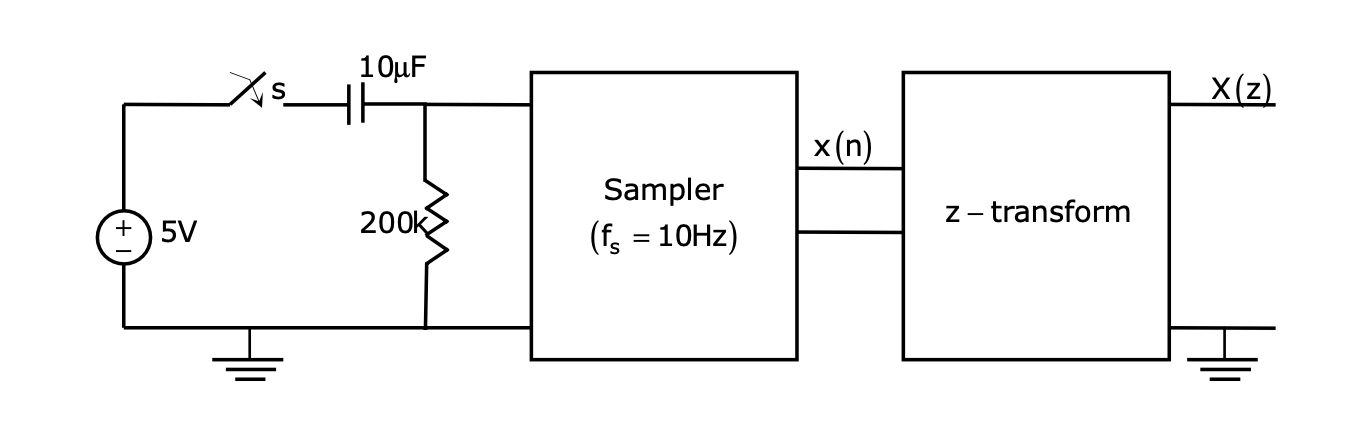
\includegraphics[width=\columnwidth]{question.png}
    \caption{question}
    \label{question}
\end{figure}
The samples x(n) (n = 0, 1, 2, $\cdots$) are given by
\begin{enumerate}
   \item $5(1 - e^{-0.05n})$
   \item $5e^{-0.05n}$
   \item $5(1 - e^{-5n})$
   \item $5e^{-5n}$
\end{enumerate}
\section*{\textbf{Solution}}
The charge q, current i, voltage V in a circuit are,
\begin{align}
    q &= cV \\
    i &= \frac{dq}{dt} = c\frac{dV}{dt} \\
    i &= \frac{V}{R} \\
    \therefore c\frac{dV}{dt} &= \frac{V}{R} 
\end{align}

In the given circuit, let V be the voltage at a given time t. From above,
\begin{align}
    c\frac{d(5-V)}{dt} &= \frac{V}{R} \\
    -c\frac{dV}{dt} &= \frac{V}{R} \\
    \frac{dV}{V} &= -\frac{dt}{Rc}
\end{align}
Integrating on both sides,
\begin{align}
    [\ln V]_5^{V} &= -\frac{1}{Rc}[t]_0^{t} \\
    \ln \frac{V}{5} &= -\frac{t}{Rc} \\
    \frac{V}{5} &= e^{-\frac{t}{Rc}} \\
    V &= 5e^{-\frac{t}{Rc}}
\end{align}
Substituting the values of
\begin{align}
    R &= 200 K = 2 \times 10^5 \Omega \\
    c &= 10 \mu F = 10^{-5} F \\
    Rc &= 2
\end{align}
We get
\begin{align}
    V = 5e^{-\frac{t}{2}} = 5e^{-0.5t} \label{eq}
\end{align}

Now, given Sampling frequency f = 10 Hz.

Sampling period T is given by
\begin{align}
    T = \frac{1}{f} = 0.1 s
\end{align}

Now, samples x[n] are obtained by replacing t with nT in \eqref{eq},
\begin{align}
    x[n] &= 5e^{-0.5nT} \\
    x[n] &= 5e^{-0.05n}
\end{align}

The samples x(n) (n = 0, 1, 2, $\cdots$) are given by $x[n] = 5e^{-0.05n}$ .

Hence, the correct answer is \textbf{Option 2}.

\end{document}